Gli esperimenti sono stati condotti variando principalmente il numero di piani da combinare e la dimensione delle immagini.
Prima dell'esecuzione dei test, sono stati generati tutti i piani e i cerchi in modo da garantire un confronto accurato
tra i diversi metodi di parallelizzazione.\\
Le dimensioni delle immagini utilizzate sono 256x256, 512x512 e 1024x1024.
Per gli esperimenti su OpenMP, il numero di piani è stato variato da 100 a un massimo di 1000,
con un incremento di 100 piani.
Nell'appendice~\ref{sec:rendering-openmp} sono riportati i risultati ottenuti con un massimo di 10000 piani.
Per gli esperimenti su CUDA invece, il numero di piani è stato variato da 1000 a un massimo di 10000,
con un incremento di 1000 piani per i test con risoluzioni 256x256 e 512x512.
Per il test con risoluzione 1024x1024, il numero di piani varia in un range più piccolo.

\subsection{OpenMP}\label{subsec:test_openmp}
In questa sezione analizziamo gli esperimenti eseguiti con la versione sequenziale e quella parallelizzata con OpenMP.
\subsubsection{Generazione dei cerchi}
Prima di tutto ci siamo occupati di osservare i risultati ottenuti con la parallelizzazione della generazione dei piani e dei cerchi.
Nella Tabella~\ref{tab:gen512} sono riportati i tempi impiegati per la generazione su immagini di dimensioni 512x512 utilizzando 16 thread.
Inoltre nelle Tabelle~\ref{tab:gen256}, ~\ref{tab:gen1024} riportate nell'appendice sono presenti gli stessi risultati ottenuti su immagini di dimensioni diverse.
\begin{table}[H]
    \centering
    \begin{tabular}{c|c|c|c|c|c|c|}
        & \multicolumn{2}{|c|}{$N = 100$} & \multicolumn{2}{|c|}{$N = 1000$} & \multicolumn{2}{|c|}{$N = 10000$} \\
        & $n=50$ & $n=500$ & $n=50$ & $n=500$ & $n=50$ & $n=500$ \\
        \hline
        Sequential (s) & 0.349 & 1.404 & 3.332 & 14.071 & 33.372 & 151.407 \\
        Parallel (s) & 0.045 & 0.180 & 0.326 & 1.701 & 3.257 & 17.310 \\
        Speedup & 7.756 & 7.800 & 10.221 & 8.272 & \textbf{10.246} & \textbf{8.747} \\
    \end{tabular}
    \caption{\label{tab:gen512}Tempi impiegati per la generazione dei cerchi e dei piani su immagini 512x512}
\end{table}
Dalle tabelle risulta evidente che si abbia un enorme vantaggio nell'utilizzo di OpenMP rispetto alla versione sequenziale.
Ciò è dovuto al fatto che la generazione dei piani e dei cerchi è un'operazione molto intensiva in termini di calcolo,
e quindi la parallelizzazione porta a un notevole miglioramento delle performance.
La parallelizzazione della generazione dei cerchi ha anche permesso di eseguire più velocemente i test seguenti.

\subsubsection{Rendering}
Per quanto riguarda l'operazione principale, ovvero il compositing dei piani, i risultati sono stati suddivisi per dimensione delle immagini.
Per ognuna di queste dimensioni è stato variato il numero di piani da combinare.\\
Le immagini 256x256 sono le più piccole testate.
In Figura~\ref{fig:omp_256} sono riportati i tempi di esecuzione (sulla sinistra) e i corrispondenti speedup
(sulla destra) per le diverse combinazioni di piani e cerchi.
\begin{figure}[H]
    \centering
    \begin{subfigure}{0.49\textwidth}
        \centering
        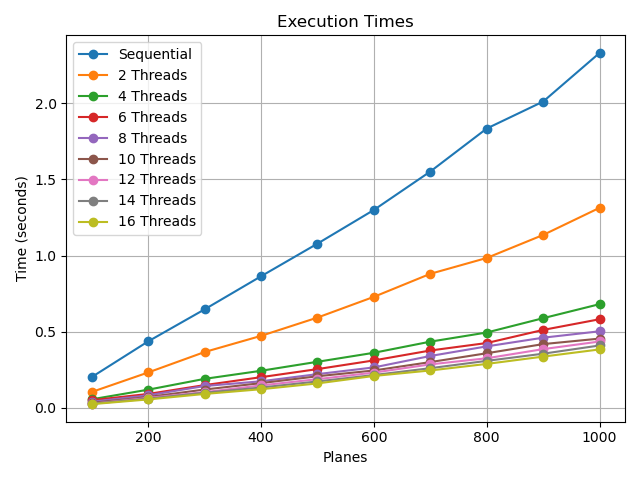
\includegraphics[width=\textwidth]{../result_16/plots/256/results_times}
    \end{subfigure}
    \begin{subfigure}{0.49\textwidth}
        \centering
        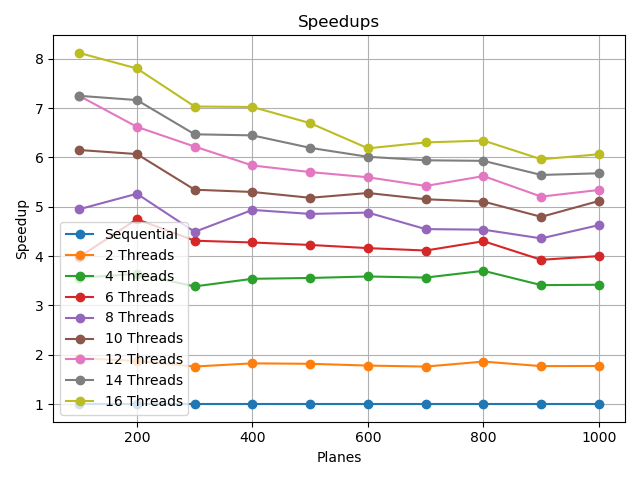
\includegraphics[width=\textwidth]{../result_16/plots/256/results_speedup}
    \end{subfigure}
    \caption{Tempi di esecuzione e speedup con OpenMP su immagini 256x256}
    \label{fig:omp_256}
\end{figure}
Appare evidente che maggiore è il numero di thread utilizzati, minore è il tempo di esecuzione.
Con 16 thread infatti si ottiene il migliore speedup che, a eccezione delle prime quantità di piani, rimane abbastanza costante per tutto l'esperimento.\\

Dopodiché abbiamo eseguito gli stessi test su immagini di dimensioni maggiori, ovvero 512x512.
I risultati in Figura~\ref{fig:omp_512}, mostrano che con immagini di dimensione maggiore, il valore dello speedup cresce leggermente.
D'altra parte possiamo notare che un numero di thread molto alto porta a una riduzione delle performance, soprattutto quando i piani diventano tanti.
\begin{figure}[H]
    \centering
    \begin{subfigure}{0.49\textwidth}
        \centering
        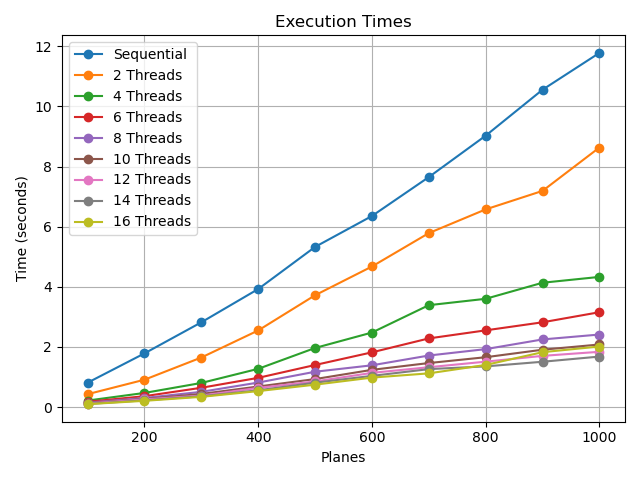
\includegraphics[width=\textwidth]{../result_16/plots/512/results_times}
    \end{subfigure}
    \begin{subfigure}{0.49\textwidth}
        \centering
        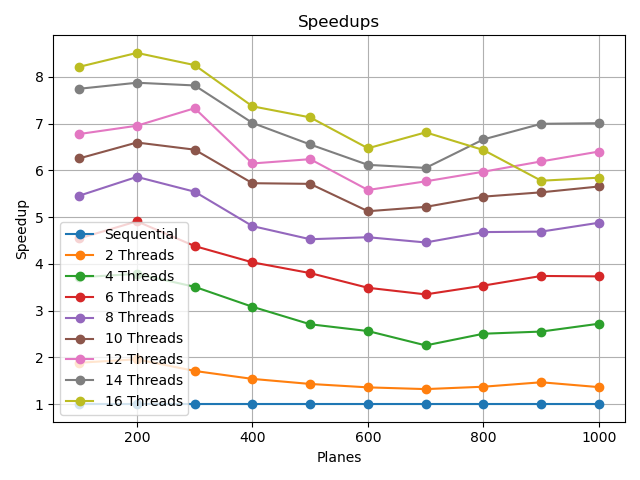
\includegraphics[width=\textwidth]{../result_16/plots/512/results_speedup}
    \end{subfigure}
    \caption{Tempi di esecuzione e speedup con OpenMP su immagini 512x512}
    \label{fig:omp_512}
\end{figure}

Infine abbiamo eseguito gli stessi esperimenti su immagini 1024x1024.
In Figura~\ref{fig:omp_1024} possiamo osservare che, con immagini così grandi, i tempi di esecuzione diventano molto maggiori.
Lo speedup però sembra non cambiare molto rispetto ai test su immagini più piccole, probabilmente a causa di un'eccessiva memoria occupata da tali piani.
\begin{figure}[H]
    \centering
    \begin{subfigure}{0.49\textwidth}
        \centering
        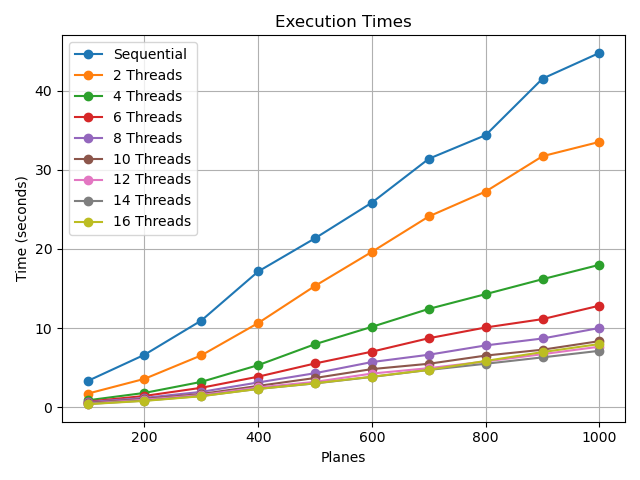
\includegraphics[width=\textwidth]{../result_16/plots/1024/results_times}
    \end{subfigure}
    \begin{subfigure}{0.49\textwidth}
        \centering
        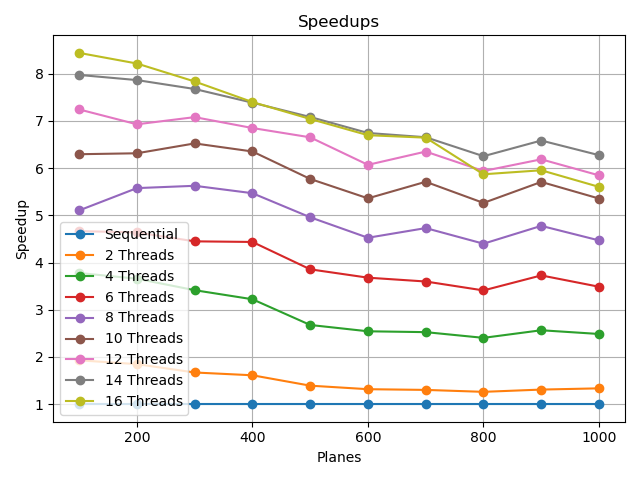
\includegraphics[width=\textwidth]{../result_16/plots/1024/results_speedup}
    \end{subfigure}
    \caption{Tempi di esecuzione e speedup con OpenMP su immagini 1024x1024}
    \label{fig:omp_1024}
\end{figure}
In tutti i casi lo speedup è rimasto abbastanza costante.
In generale con un numero maggiore di thread si sono ottenuti risultati migliori, ma un numero molto alto di thread
affiancato a una grande quantità di memoria utilizzata, ha determinato un peggioramento delle performance.

\subsection{CUDA}\label{subsec:test_cuda}
Passiamo adesso ad analizzare gli esperimenti eseguiti utilizzando CUDA come metodo di parallelizzazione.
Ovviamente ci aspettiamo valori di speedup molto maggiori dei precedenti, dato l'utilizzo della GPU a disposizione.

\subsubsection{Dimensione dei thread-blocks}
Come abbiamo visto, per la costruzione della griglia e dei blocchi della GPU è necessario scegliere una dimensione appropriata.
Abbiamo quindi eseguito degli esperimenti per determinare la dimensione ottimale dei thread-blocks.
In particolare, sappiamo che conviene utilizzare un numero di thread per blocco multiplo di 32 e relativamente grande,
in modo da sfruttare al meglio le istanze degli warp.
Allo stesso tempo la nostra GPU permette un massimo di 1024 thread per blocco.
Abbiamo quindi testato le performance con blocchi di dimensione 8x8, 16x16 e 32x32.
I risultati riportati in Tabella~\ref{tab:cuda_blocks} mostrano i tempi di esecuzione dell'operazione di rendering al
variare della dimensione delle immagini e del numero di piani.
\begin{table}[H]
    \centering
    \begin{tabular}{c|c|c|c|c|c|c|}
        & \multicolumn{6}{|c|}{Dimensione dell'immagine} \\
        & \multicolumn{2}{|c|}{$256x256$} & \multicolumn{2}{|c|}{$512x512$} & \multicolumn{2}{|c|}{$1024x1024$} \\
        & $N=500$ & $N=5000$ & $N=500$ & $N=5000$ & $N=500$ & $N=2000$ \\
        \hline
        $8x8$ & 0.024 & 0.189 & 0.086 & 0.884 & 0.252 & 2.507\\
        $16x16$ & \textbf{0.021} & \textbf{0.157} & 0.073 & \textbf{0.645} & \textbf{0.249} & 1.214\\
        $32x32$ & 0.022 & 0.161 & \textbf{0.066} & 0.657 & \textbf{0.249} & \textbf{1.107} \\
    \end{tabular}
    \caption{\label{tab:cuda_blocks}Tempi (secondi) impiegati per il rendering con diverse dimensioni dei thread-blocks di CUDA}
\end{table}

Come ci aspettavamo, i blocchi 8x8 sono risultati in tutti i casi quelli meno performanti.
I blocchi 16x16 sembrano fare leggermente meglio di quelli 32x32, anche se entrambi determinano tempi di esecuzione simili.
Dunque per tutti i prossimi esperimenti abbiamo utilizzato blocchi 16x16, ovvero da 256 threads.

\subsubsection{Rendering}
Poiché abbiamo notato che la dimensione ottimale dei thread-blocks è 32x32, abbiamo eseguito tutti i prossimi test seguendo questa configurazione.
Anche in questo caso gli esperimenti sono suddivisi sulla base della dimensione delle immagini.\\
Come nel caso di OpenMP, il primo test è stato eseguito su immagini 256x256 e il numero di piani è stato variato tra un minimo di 1000 e un massimo di 10000.
I risultati sono riportati in Figura~\ref{fig:cuda_256}.
\begin{figure}[H]
    \centering
    \begin{subfigure}{0.49\textwidth}
        \centering
        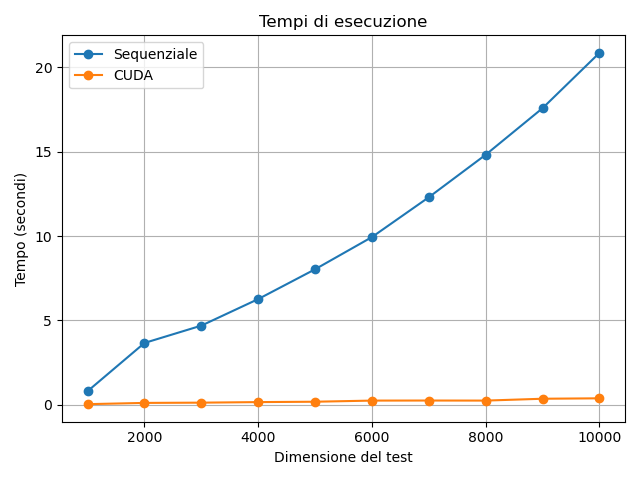
\includegraphics[width=\textwidth]{../results/plots/256/cuda_times}
    \end{subfigure}
    \begin{subfigure}{0.49\textwidth}
        \centering
        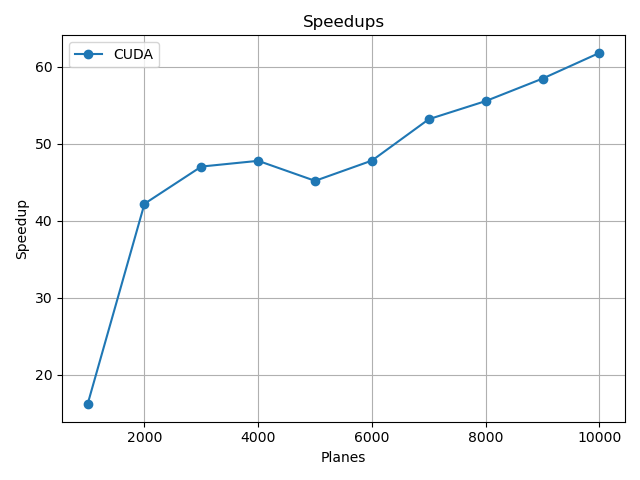
\includegraphics[width=\textwidth]{../results/plots/256/cuda_speedup}
    \end{subfigure}
    \caption{Tempi di esecuzione e speedup con CUDA su immagini 256x256}
    \label{fig:cuda_256}
\end{figure}
Come ci aspettavamo, il tempo di esecuzione è molto minore rispetto a quello ottenuto eseguendo le operazioni sulla CPU.
Lo speedup aumenta man mano che cresce il numero di piani combinati e si ottengono tempi circa 60 volte minori rispetto
alla versione sequenziale quando i piani arrivano intorno al loro massimo. \\

Di seguito invece abbiamo riportati i risultati degli stessi esperimenti eseguiti su immagini 512x512.
\begin{figure}[H]
    \centering
    \begin{subfigure}{0.49\textwidth}
        \centering
        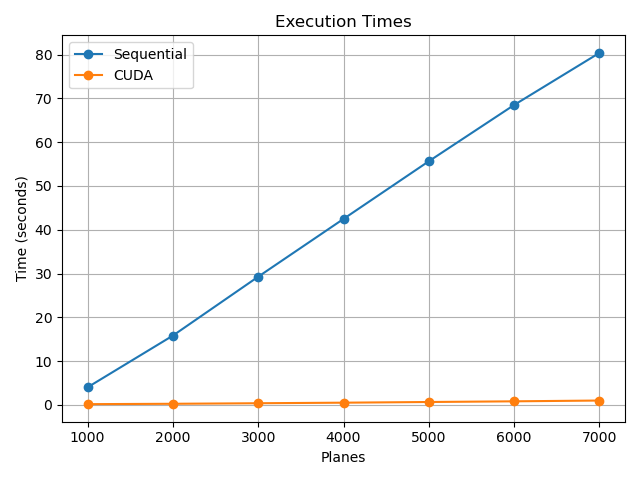
\includegraphics[width=\textwidth]{../results/plots/512/cuda_times}
    \end{subfigure}
    \begin{subfigure}{0.49\textwidth}
        \centering
        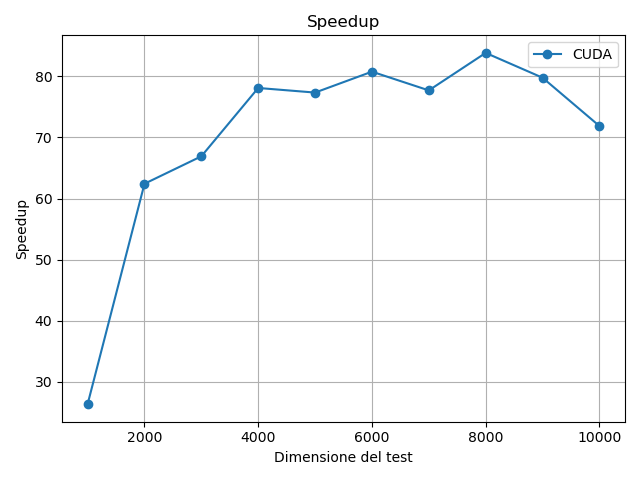
\includegraphics[width=\textwidth]{../results/plots/512/cuda_speedup}
    \end{subfigure}
    \caption{Tempi di esecuzione e speedup con CUDA su immagini 512x512}
    \label{fig:cuda_512}
\end{figure}
Essendo aumentata la quantità di pixel da elaborare, lo sfruttamento della GPU è diventato ancora più vantaggioso.
I tempi impiegati per il compositing sono ovviamente più lunghi dei precedenti, specialmente per la versione sequenziale,
dunque anche lo speedup migliora rispetto alle immagini più piccole e tocca un massimo di 85 intorno ai 4000-6000 piani.\\

Infine abbiamo eseguito gli stessi esperimenti su immagini 1024x1024, i cui risultati sono mostrati in Figura~\ref{fig:cuda_1024}.
In questo caso, a causa di limitazioni computazionali della GPU a disposizione, abbiamo potuto eseguire i test sono con un numero minore di piani.
I risultati che abbiamo ottenuto, fino al massimo di valori testati, rimangono coerenti con quelli ottenuti in precedenza.
Ci possiamo ovviamente aspettare che con un numero di pixel ancora maggiore, lo speedup crescerebbe maggiormente rispetto ai casi sopra.
\begin{figure}[H]
    \centering
    \begin{subfigure}{0.49\textwidth}
        \centering
        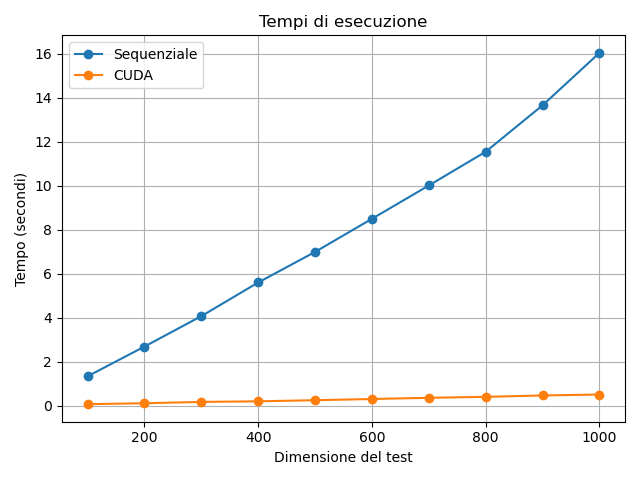
\includegraphics[width=\textwidth]{../results/plots/1024/cuda_times}
    \end{subfigure}
    \begin{subfigure}{0.49\textwidth}
        \centering
        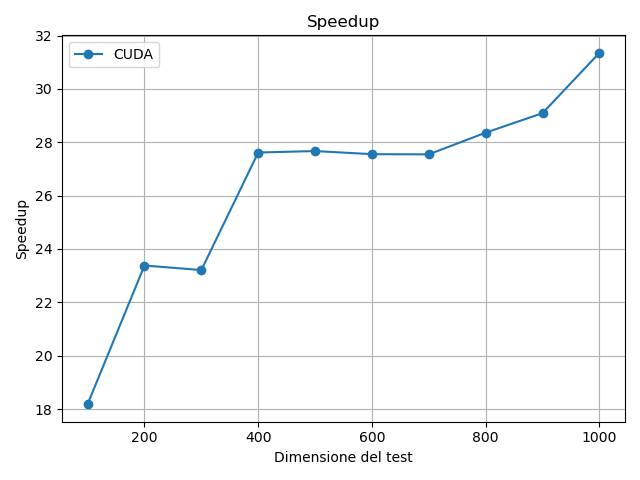
\includegraphics[width=\textwidth]{../results/plots/1024/cuda_speedup}
    \end{subfigure}
    \caption{Tempi di esecuzione e speedup con CUDA su immagini 1024x1024}
    \label{fig:cuda_1024}
\end{figure}

\subsubsection{Utilizzo dei burst di memoria (CUDA-Color)}
Poiché potrebbe essere vantaggioso sfruttare i burst di memoria per migliorare le performance, abbiamo eseguito degli
esperimenti per valutare l'efficacia di questa tecnica nel caso del Rendering.
A differenza del metodo precedente, abbiamo utilizzato un kernel diverso.
L'array dei piani passato in ingresso è stato riordinato in modo da avere ogni canale di ogni pixel separato.
In questo modo tale canale, gestito da un solo thread, sarà rappresentato dal suo valore su tutti i piani in maniera contigua.
Ciò dovrebbe permettere di sfruttare il caricamento in burst dalla memoria globale della GPU.
\lstinputlisting[language=c++, firstline=255, lastline=275,label={lst:cuda-color}]{../src/renderer.cu}
Come è possibile osservare nello snippet di codice sopra, in questo caso l'array contenente le informazioni dei piani
sarà di tipo $uchar$ invece che $uchar4$ e ovviamente il codice del kernel è leggermente diverso.
Si può notare che nel ciclo $for$ viene sfruttata la memoria contigua per caricare i valori dei piani in un registro,
in modo da poterli utilizzare per il calcolo del colore del pixel.
I risultati ottenuti sono riportati in Figura~\ref{fig:cuda_color}.
\begin{figure}[H]
    \centering
    \begin{subfigure}{0.49\textwidth}
        \centering
        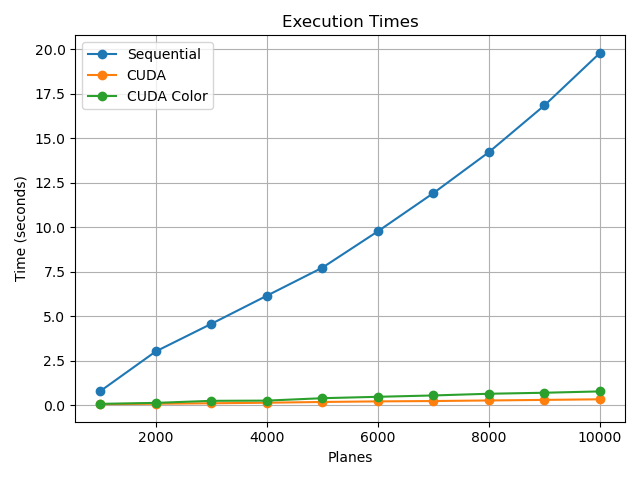
\includegraphics[width=\textwidth]{../results/plots/256/cuda_color_times}
    \end{subfigure}
    \begin{subfigure}{0.49\textwidth}
        \centering
        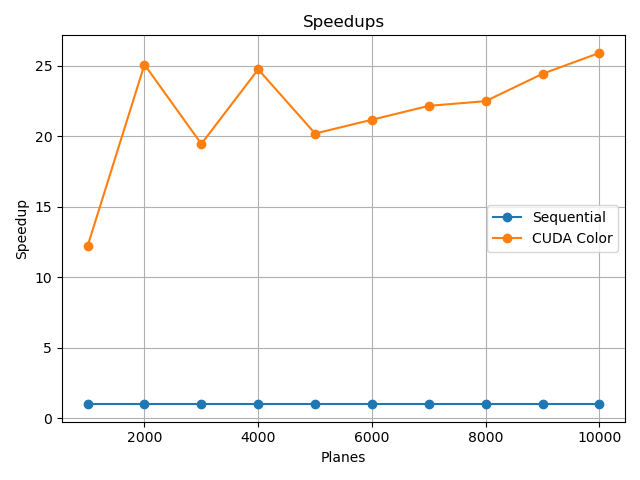
\includegraphics[width=\textwidth]{../results/plots/256/cuda_color_speedup}
    \end{subfigure}
    \caption{Tempi di esecuzione e speedup con CUDA-Color su immagini 256x256}
    \label{fig:cuda_color}
\end{figure}
A differenza di ciò che ci aspettavamo, i risultati sono a favore della versione che abbiamo visto finora.
Ciò può dipendere dal fatto che in questo caso ogni thread legge un elemento $uchar$ per volta e si trova quindi a
eseguire il quadruplo delle letture dalla memoria globale rispetto alla versione precedente.

\subsubsection{Copia dei dati in GPU}
In tutti gli esperimenti che abbiamo eseguito, non abbiamo tenuto conto del tempo impiegato per la copia dei dati
dalla CPU alla scheda grafica e viceversa.
Questo è un aspetto molto importante da considerare, in quanto potrebbe influenzare notevolmente le performance.
In Figura~\ref{fig:cuda_memcpy} sono mostrate le differenze tra i tempi di esecuzioni visti finora e quelli complessivi
della copia dei dati da e verso la GPU.
\begin{figure}[H]
    \centering
    \begin{subfigure}{0.49\textwidth}
        \centering
        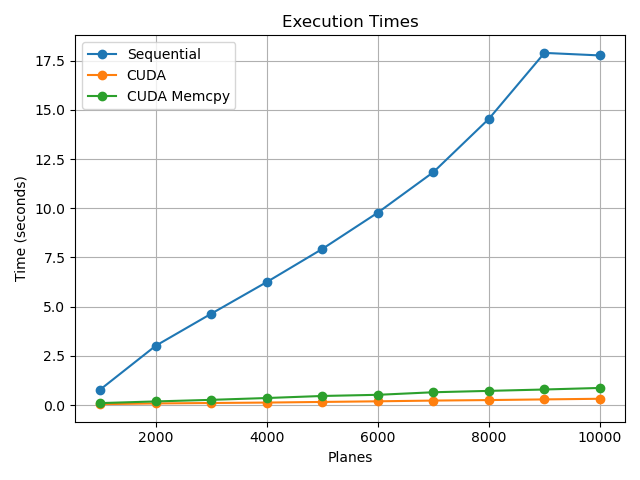
\includegraphics[width=\textwidth]{../results/plots/256/cuda_memcpy_times}
    \end{subfigure}
    \begin{subfigure}{0.49\textwidth}
        \centering
        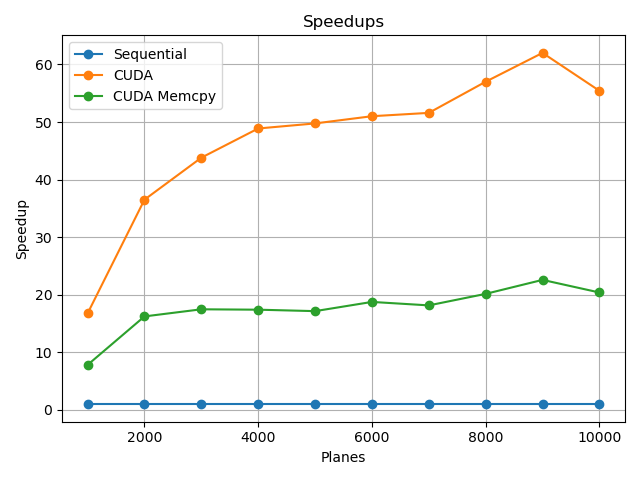
\includegraphics[width=\textwidth]{../results/plots/256/cuda_memcpy_speedup}
    \end{subfigure}
    \caption{Tempi di esecuzione e speedup con CUDA-Color su immagini 256x256}
    \label{fig:cuda_memcpy}
\end{figure}
Come ci aspettavamo, se consideriamo il tempo impiegato per il passaggio dei dati, i tempi si allungano e lo
speedup cala significativamente.
Ciò è indubbiamente dovuto al fatto che la quantità di dati scambiati tra l'host e la GPU è molto pesante e su di essa
vengono poi eseguite operazioni relativamente leggere.

